\chapter{Estado da Arte} 
\label{chap:Chapter02} 

\section{Sistema Braille}

\subsection{História do Braille}

Braille é um sistema de escrita tátil que permite às pessoas com deficiência visual ler e escrever de forma independente. Desenvolvido pelo francês Louis Braille no século XIX \parencite{REF02}, o sistema utiliza uma série de pontos em relevo dispostos em células de seis pontos. Com isso, o Braille é capaz de representar letras, números, símbolos matemáticos e até mesmo partituras musicais. 

\begin{figure}[h]
    \centering
    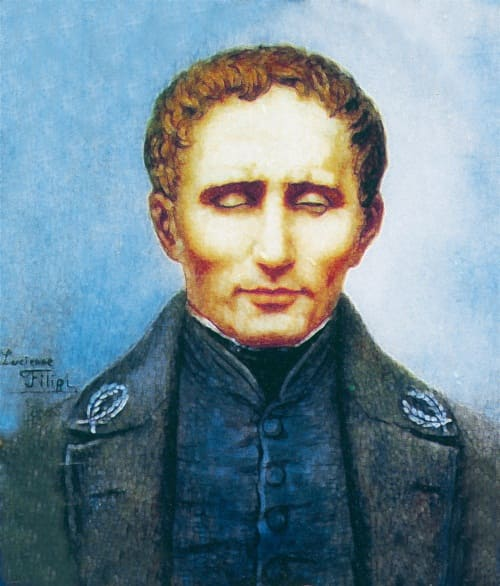
\includegraphics[scale=0.5]{ch02/assets/louis-braille.jpg}
    \decoRule
    \caption[Louis Braille]{Louis Braille, criador do Sistema Braille \parencite{IMG01}}
    \label{fig:ch02-braille-history-louis-braille}
\end{figure}

Na época, era utilizado o sistema Valentin Haüy \parencite{REF03}, que consistia em imprimir livros com a fonte bem ampliada e em relevo, possibilitando assim a leitura, mas não a escrita. Louis decidiu então buscar uma solução em um método que permitisse de forma prática e com poucas combinações a leitura e escrita para pessoas com deficiência visual.

Em 1824, Louis concluiu o desenvolvimento da base de seu sistema, aos 15 anos de idade. Ao longo dos anos continuou aprimorando, e em 1839 sua última publicação explicando o seu método foi muito bem recebida por parte dos alunos do Instituto Nacional para Jovens Cegos. Então, em 1843, o sistema Braille foi oficialmente adotado pelo instituto e passou a ser difundido por toda a Europa \parencite{REF03}.

Em 1852, Louis Braille faleceu aos 43 anos, devido a complicações de tuberculose. Louis deixou um legado duradouro \parencite{REF03}. Seu sistema de escrita tátil revolucionou a comunicação de pessoas com deficiência visual. Além de permitir o acesso à informação escrita, o sistema Braille até hoje promove igualdade de oportunidades educacionais e profissionais, permitindo seus usuários participarem ativamente da sociedade.

\subsection{Funcionamento do Sistema Braille}

O Braille é composto por unidades básicas denominadas de “celas” ou “células” que são compostas por uma matriz de pontos dispostos em duas colunas verticais. Cada célula pode conter de zero a seis pontos, numerados de 1 a 6. Os pontos são organizados em duas colunas, com três pontos em cada coluna. Assim, os pontos da esquerda de cima para baixo são os pontos 1, 2 e 3, e os da direita são os pontos 4, 5 e 6 \parencite{REF04}.

\begin{figure}[h]
    \centering
    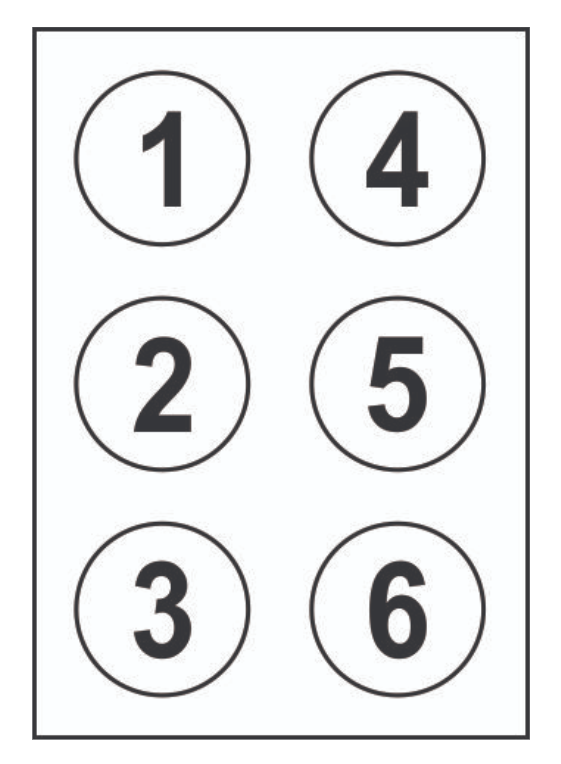
\includegraphics[scale=0.5]{ch02/assets/braille-cell.png}
    \decoRule
    \caption[Cela Braille]{Cela Braille}
    \label{fig:ch02-braille-cell}
\end{figure}

Cada combinação de pontos dentro da cela pode representar um caractere específico ou uma convenção adotada no Braille. Existem um total de 64 combinações possíveis, incluindo a cela totalmente vazia. Celas individuais ou a combinação de celas permitem o Braille representar letras do alfabeto, números, símbolos matemáticos, sinais de pontuação, palavras, frases e até mesmo textos inteiros \parencite{REF05}.

\begin{figure}[h]
    \centering
    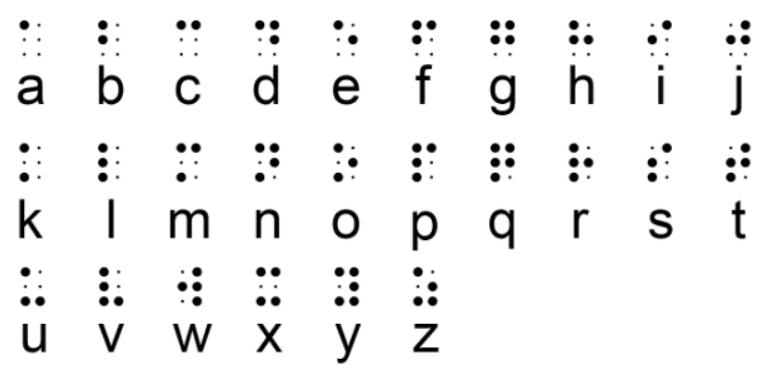
\includegraphics[scale=0.5]{ch02/assets/braille-alphabet.png}
    \decoRule
    \caption[Alfabeto em Braille]{Alfabeto em Braille}
    \label{fig:ch02-braille-alphabet}
\end{figure}

Para ler um texto Braille, uma pessoa utiliza as pontas dos dedos para sentir os pontos em relevo em alguma superfície. Cada cela é sentida e lida individualmente e, com prática, os leitores de Braille são capazes de fazer a leitura rapidamente. Já para a escrita em Braille, há diversas técnicas. O uso de uma reglete e um punção é uma das formas mais comuns de se escrever em Braille, onde o usuário pressiona pontos em uma folha de papel especial para criar pontos em relevo.

A máquina de escrever em Braille também é uma das formas mais comuns e tradicionais de gerar textos em Braille. Ela é especialmente projetada para permitir que pessoas cegas ou com baixa visão escrevam em Braille de forma eficiente e precisa. Seu funcionamento se assemelha a máquina de escrever convencional, porém com menos teclas e produzindo pontos em relevo para formar as celas Braille.

\section{Máquina Braille}

\subsection{Visão Geral}

Em 1892, o americano Frank Haven Hall pensou na primeira máquina própria para escrever em Braille. Em 1951, surgiu a Máquina Perkins, desenvolvida por um carpinteiro que trabalhava na Perkins School for the Blind, David Abraham. A máquina tem um funcionamento bem simples e intuitivo, além de muito parecido com uma máquina de escrever tradicional

\begin{figure}[h]
    \centering
    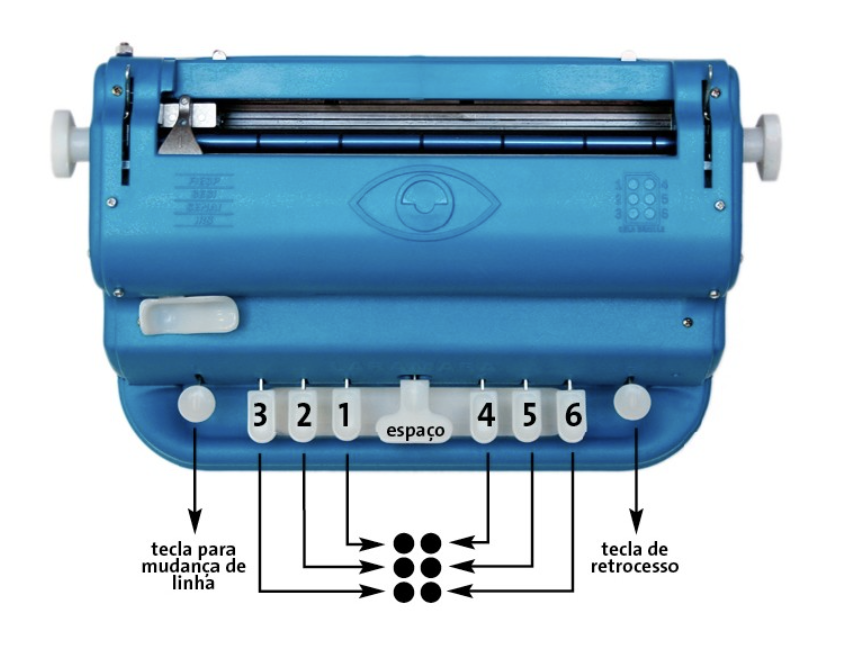
\includegraphics[scale=0.5]{ch02/assets/braille-typewriter.png}
    \decoRule
    \caption[Máquina Braille]{Máquina Braille com as teclas sinalizadas}
    \label{fig:ch02-braille-typewriter}
\end{figure}

Consistem em sete teclas principais, sendo que seis delas representam cada ponto de uma cela Braille e uma que representa uma cela vazia. Quando uma tecla é pressionada, o ponto correspondente é perfurado em um papel colocado atrás da máquina, criando assim o texto em Braille. Algumas máquinas também incluem características adicionais, como ajuste de espaçamento entre as células e a capacidade de produzir caracteres em negrito para ênfase.

Essas máquinas são muito importantes para pessoas com deficiência visual, seu uso se torna crucial no meio acadêmico e profissional, pois lhes permite criar documentos e ter acesso a informações de forma independente. As máquinas Braille vêm tendo avanços tecnológicos, com máquinas cada vez mais sofisticadas e integradas a outros dispositivos eletrônicos.

\subsection{Valores da Máquina Braille}
\label{sec:ch02_Valores_da_Maquina_Braille}

Apesar da importância da máquina Braille para as pessoas com deficiência visual, um dos principais obstáculos para a aquisição desse equipamento é o seu custo elevado. Uma busca no site oficial da Perkins, uma das mais renomadas fabricantes desse dispositivo, mostra que as máquinas de escrever em Braille estão longe de serem acessíveis para a maioria das pessoas, pois os preços são bem expressivos. Por exemplo, uma Máquina Braille comum é vendida por \$810, enquanto uma Máquina Braille Inteligente chega a \$2.195,00. Convertendo esses valores para real e euro, temos que a Máquina Braille Comum custa R\$3.996,54 ou 746,78€. Já a Máquina Braille Inteligente custa R\$10.829,91 ou 2.023,61€.

Diante disso, torna-se compreensível que a maioria indivíduos com deficiência visual tenham dificuldade ao tentar adquirir uma Máquina Braille. O alto custo desse equipamento torna a compra praticamente inviável para muitas pessoas, especialmente aquelas com recursos financeiros mais limitados. Instituições de ensino de Braille também se tornam afetadas nesse cenário, já que não é muito viável a compra de vários exemplares para disponibilizar para os alunos. Assim, a alternativa de investir em outras tecnologias, como computadores ou notebooks, parece ser mais atrativa.

\section{Trabalhos relacionados}

\subsection{BrailleType}

No BrailleType \parencite{REF06}, a interface consiste em 6 botões ordenados em 2 colunas. Esse botões são colocados nas bordas e cantos da tela para facilitar sua localização. Os pontos são escolhidos um por um em qualquer ordem com confirmação de áudio. O BrailleType permite que o usuário cego insira texto como se estivesse escrevendo Braille usando o tradicional código matricial de 6 pontos.

\begin{figure}[h]
    \centering
    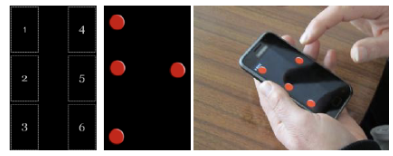
\includegraphics{ch02/assets/brailletype.png}
    \decoRule
    \caption[Interface do BrailleType]{Tela principal do BrailleType à esquerda. Ao centro mostra a letra 'r' marcada e pronta para ser confirmada. À direita um usuário escrevendo a letra 'r' no BrailleType. \parencite{REF06}}
    \label{fig:ch02-brailletype}
\end{figure}

Todas as interações com BrailleType são feitas usando apenas um único dedo. Sempre que um usuário pressiona ou arrasta um dedo para um novo ponto, o número do ponto correspondente é anunciado de forma audível, mas o ponto não é selecionado imediatamente. Há um pequeno tempo a se esperar para evitar seleções involuntárias do usuário. Este tempo pode ser facilmente configurado, permitindo que um usuário mais experiente diminua ou elimine a espera. 

Então, para marcar um ponto na célula Braille, o usuário deve tocar no alvo desejado e aguardar um sinal sonoro de confirmação. Repetindo o processo em um ponto já marcado o remove e informa ao usuário por meio de feedback de áudio. Após marcar todos os pontos necessários para um caractere Braille, na ordem que o usuário desejar, um duplo toque em qualquer parte da tela confirma a inserção. Se o usuário tentar aceitar uma combinação incorreta de pontos, a matriz Braille será apagada e um som de erro será reproduzido.

Esta aplicação oferece uma abordagem menos estressante com dispositivos com tela sensível ao toque, reduzindo o número de toques na tela. Ao reduzir o número de erros e permitir que o usuário tenha sucesso, sua confiança aumenta. Além de aproveitar as capacidades daqueles que usam Braille regularmente, também permite que aqueles que não o fazem aprendam ou mantenham o uso do Braille através de interações diárias simples.

\subsection{SingleTapBraille}

O principal objetivo do SingleTapBraille \parencite{REF07} foi desenvolver um novo método de entrada de texto que elimine a necessidade de os usuários encontrarem locais específicos para inserir letras, permitindo que as informações sejam inseridas de maneira rápida e eficaz usando um único polegar ou dedo. O objetivo buscou identificar as melhores funcionalidades para usuários que estão restritos a usar apenas uma mão para realizar tarefas em seu dispositivo móvel. Uma conclusão preliminar do estudo foi que a maioria dos usuários preferiria usar o polegar para interagir com telas sensíveis ao toque.

O sistema foi desenvolvido com base em padrões braille, cada um com duas colunas e três linhas. O método de entrada permite que os usuários insiram pontos da esquerda para a direita, que é a forma como os usuários cegos leem braille. Cada ponto braille é ativado individualmente com um único toque na tela. Por exemplo, se o usuário tocar uma vez em qualquer parte da tela, isso representará a letra 'a' e significa que o usuário "pressionou" o primeiro ponto em braille. Quando o usuário parar de tocar na tela por um curto intervalo, o padrão braille é interpretado, a caractere resultante é digitado e o software o lê. 

Com o SingleTapBraille, os usuários podem segurar o celular com uma mão porque precisam apenas de um dedo ou do polegar para inserir pontos braille na tela sensível ao toque. Nessa abordagem, é analisado a relação entre os pontos ativos em cada caractere braille com base em suas coordenadas e na distância entre cada ponto e os seguintes. Por exemplo, se o usuário der dois toques um abaixo do outro, isso representará a letra 'b', pois o usuário "pressionou" o primeiro e o segundo ponto em braille. A aplicação analisará a relação entre esses dois toques, identificará o símbolo pretendido e o exibirá na tela.

\begin{figure}[h]
    \centering
    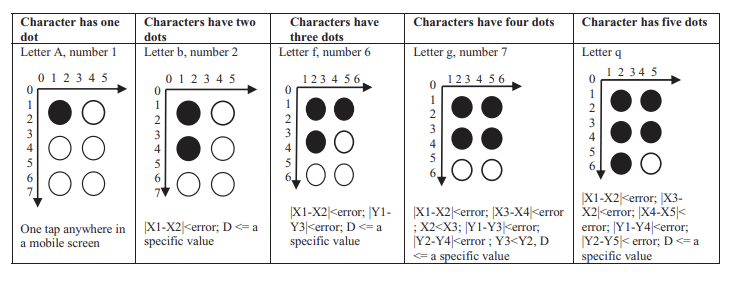
\includegraphics{ch02/assets/categorization-of-braille.png}
    \decoRule
    \caption[Categorização de coordenadas do SingleTapBraille]{Amostra de categorização de caracteres braille com base no número de pontos \parencite{REF07}}
    \label{fig:ch02-categorization-of-braille}
\end{figure}

O principal conceito por trás do método de entrada é o agrupamento de pontos braille ativados para cada caractere. Quando o usuário para de tocar na tela por um curto intervalo, nosso algoritmo agrupa os toques inseridos e os interpreta com base no número de pontos. O algoritmo processa as coordenadas de cada ponto, bem como o espaço entre cada ponto e o seguinte.

A principal vantagem é que não restringe os usuários, exigindo que encontrem um objeto específico na tela, em vez disso, permite que eles toquem nos pontos braille em qualquer lugar da tela com base em padrões braille. Não possui botão ou outro tipo de controle que exija que o usuário toque ou clique com precisão em pontos específicos. É totalmente acionado por gestos e possui uma saída de voz correspondente. 

É importante ressaltar que a aplicação pode ser usada tanto por pessoas estacionárias quanto por pessoas em movimento. Existem algumas operações de digitação, como espaço e backspace, que o teclado braille não apresenta utilizando pontos braille, pois possuem botões específicos na máquina braille que realizam essas funções, e que foi simulado através de gestos do usuário.

\begin{figure}[h]
    \centering
    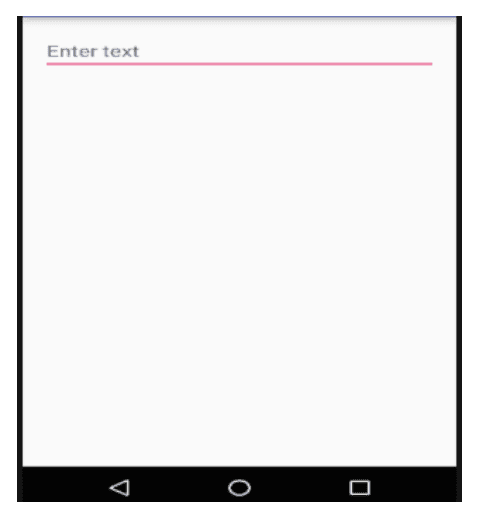
\includegraphics[scale=0.5]{ch02/assets/singletapbraille-gui.png}
    \decoRule
    \caption[Interface do SingleTapBraille]{Interface do SingleTapBraille \parencite{REF07}}
    \label{fig:ch02-singletapbraille-gui}
\end{figure}

O SingleTapBraille foi projetado para usuários que conhecem braille e sabem ler e escrever em braille, além de terem experiência com dispositivos touchscreen. Esta aplicação tem como objetivo melhorar a velocidade de digitação e edição na tela do celular, ao mesmo tempo que minimiza a taxa de erros.

\subsection{Brailendo}

O Brailendo \parencite{REF09} é uma ferramenta criada com o propósito de auxiliar alunos e professores a aprenderem e praticarem de forma autônoma o Sistema Braille em suas várias representações do Braille, como textual, matemático, musical, entre outros.

Em sua interface principal, é possível digitar normalmente no teclado, e a medida que o usuário digita aparece as células equivalentes em Braille, assim como os pontos em forma de números, e o texto em metabraille.

Nessa mesma interface, o Braillendo dá a possibilidade de digitar usando as teclas 'F', 'D', 'S', 'J', 'K', 'L' do teclado computador do usuário, simulando o uso de uma Máquina Braille real.

\begin{figure}[h]
    \centering
    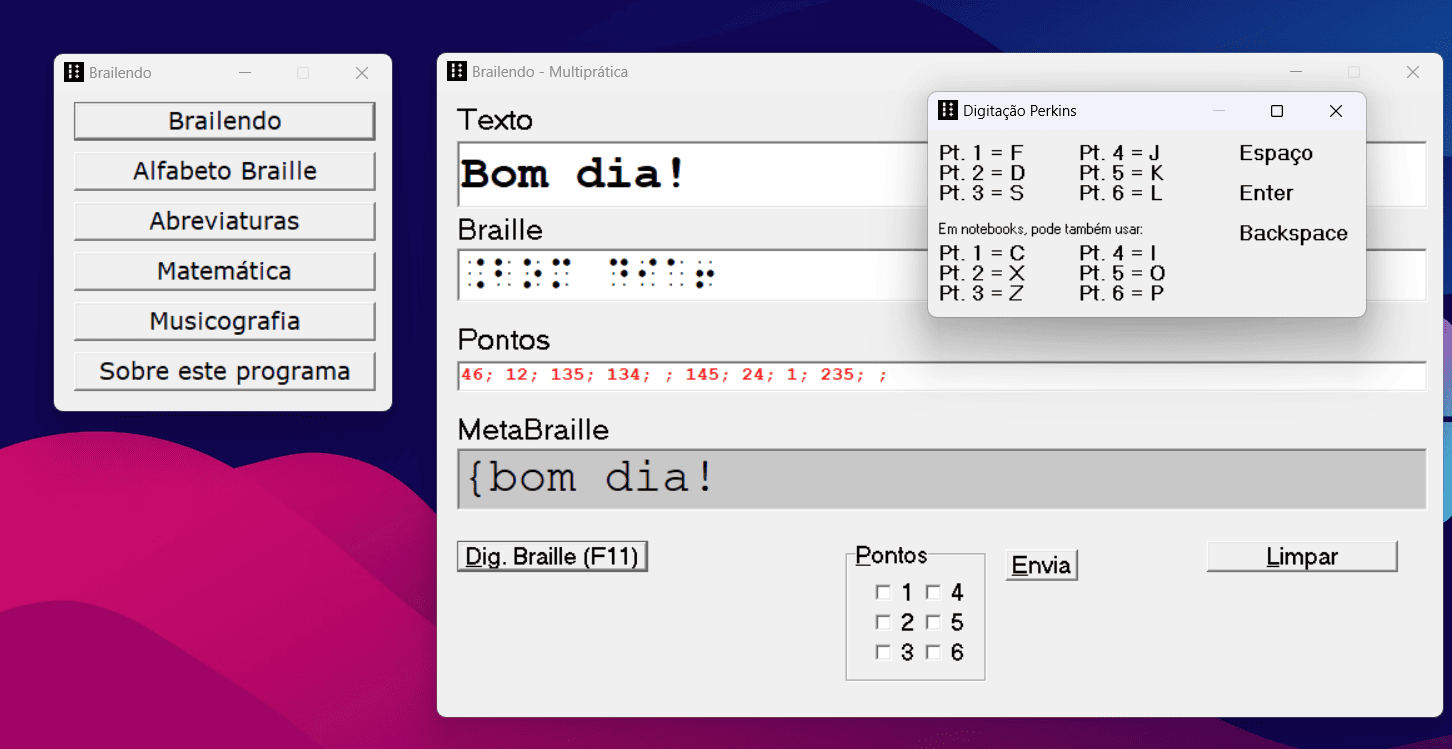
\includegraphics[scale=0.3]{ch02/assets/brailendo-gui.png}
    \decoRule
    \caption[Interface do Brailendo]{Interface do Brailendo}
    \label{fig:ch02-brailendo-gui}
\end{figure}

Além disso, a aplicação disponibiliza várias outras interfaces que contém todas células Braille, funções que permitem aprender e praticar a mecânica de criação de expressões matemáticas em braille, funções que permitem a conversão direta entre expressões escritas em asciiMath e braille, além de uma opção de musicografia em braille, onde aparece um teclado virtual, e ao selecionar as teclas, aparece a representação em notas musicais e também em Braille. É possível reproduzir o som após escolher uma combinação de notas musicais.

\subsection{Braillearning}

O Braillearnig \parencite{REF08} foi desenvolvido para auxiliar pessoas com deficiência visual no uso e aprendizado da Máquina Braille, além de ajudá-los na memorização do alfabeto Braille, sendo esse software um alternativa gratuita à Máquina Braille.

Para simular os botões da Máquina Braille, o Braillearning utiliza as teclas 'F', 'D', 'S', 'J', 'K', 'L' do teclado computador do usuário, simulando as teclas que representam os pontos 1, 2, 3, 4, 5 e 6 na máquina física. Assim, a ferramenta simula o uso real de uma Máquina Braille. O resultado da combinação de teclas pressionadas é exibido na tela com a letra, número ou símbolo equivalente no texto a tinta.

\begin{figure}[h]
    \centering
    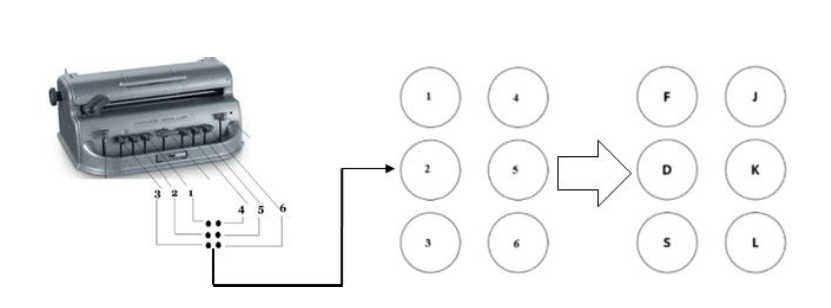
\includegraphics[scale=0.5]{ch02/assets/braillearning-keys.png}
    \decoRule
    \caption[Teclas do Braillearning]{Máquina de escrever em Braille e teclas utilizadas no Braillearning \parencite{REF08}}
    \label{fig:ch02-braillearning-modes}
\end{figure}

O Braillearning possui três modos de uso: tutorial, palavra e livre.

No modo tutorial o usuário recebe em formato de áudio e imagem um caractere, e então o usuário tem que pressionar as teclas que formam o caractere equivalente em Braille. Este modo é focado no aprendizado do Braille, por isso, oferece atalhos para dicas, no caso do usuário precisar.

O modo palavra sorteia uma palavra e a exibe, o usuário então deve digitar essa palavra usando a simulação das teclas da Máquina Braille. Enquanto o usuário vai acertando ele recebe como saída o caractere digitado e um efeito sonoro de sucesso. No caso de erro, um efeito sonoro de erro é reproduzido ao usuário, e então ele pode tentar novamente fazer a combinação de letras.

O modo livre permite ao usuário digitar livremente o que ele quiser no simulador. É o modo que mais se assemelha ao uso real da Máquina Braille.

Após os Braillearning se mostrou uma ferramenta que simula bem o uso real da Máquina Braille, podendo ser utilizada tanto por usuários videntes quanto por usuários com deficiência visual. O simulador pode ser usuado tanto para aprendizado do Braille e Máquina Braille, quando para apenas praticar o seu uso.

\begin{figure}[h]
    \centering
    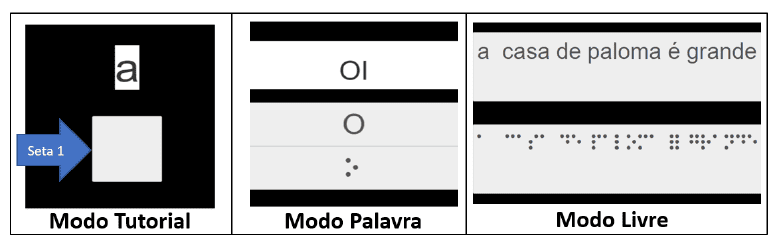
\includegraphics[scale=0.5]{ch02/assets/braillearning-modes.png}
    \decoRule
    \caption[Modos do Braillearning]{Modos de operação do Braillearning \parencite{REF08}}
    \label{fig:ch02-braillearning-modes}
\end{figure}

Apesar da semelhança, o contato com a Máquina Braille real continua sendo indispensável, visto que é necessário a prática da leitura do Braille com as mãos, o que não é possível com o Braillearning, sendo possível apenas a leitura com os outros ou ouvindo os leitores de tela.

\subsection{Braille Fácil}

O Braille Fácil \parencite{REF09} é uma ferramenta criada para facilitar e agilizar a criação de uma impressão em Braille. O texto a ser impresso pode ser digitado diretamente na aplicação ou pode ser importado a partir de um arquivo de texto simples. Com o texto na aplicação, o usuário pode visualizar com será a impressão. 

O Braille Fácil se encarrega de converter cada caractere para os sinal Braille equivalente. O programa gera arquivos de impressão com compatibilidade para diversas impressoras. Além de agilizar o processo de geração de números de páginas, gráficos e controle de margens.

\begin{figure}[h]
    \centering
    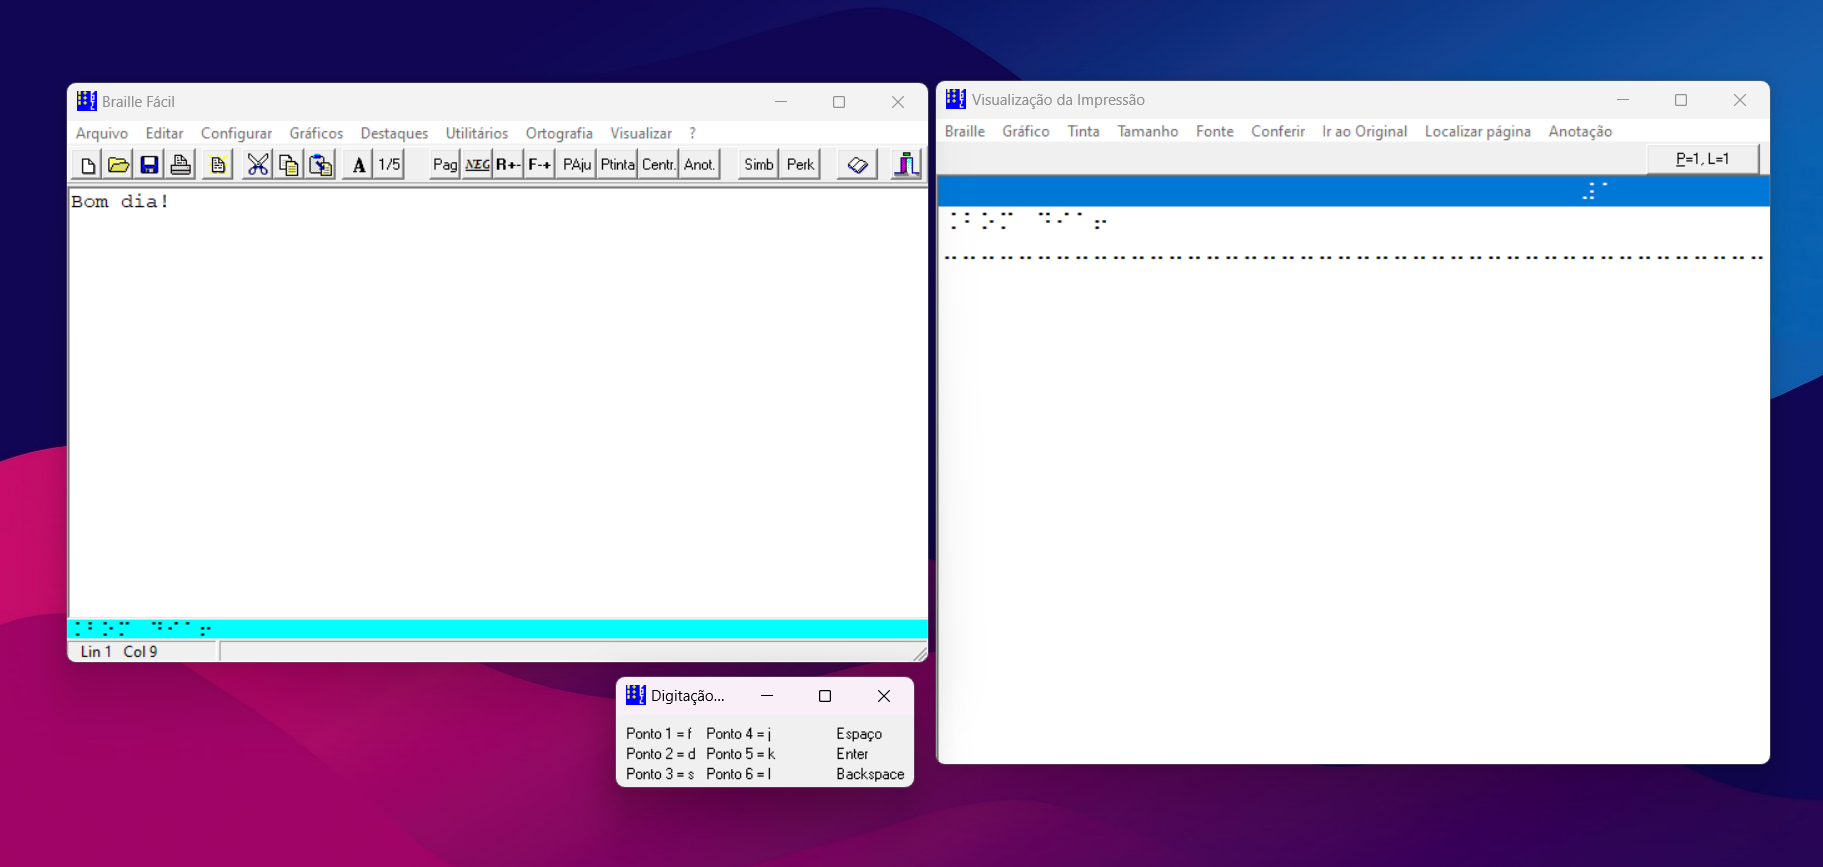
\includegraphics[scale=0.3]{ch02/assets/braille-facil-gui.png}
    \decoRule
    \caption[Interface do Braille Fácil]{Interface do do Braille Fácil}
    \label{fig:ch02-braille-facil-gui}
\end{figure}

Também dispõe de uma funcionalidade de escrita simulando uma Máquina Braille utilizando as teclas 'F', 'D', 'S', 'J', 'K', 'L' do teclado computador. Assim, um usuário cego pode digitar na aplicação como se estivesse usando uma Máquina Braille real.

\section{Aplicações Simuladoras da Máquina Braille}

\subsection{Duxbury Systems: Perky Duck}

A aplicação Perky Duck é uma ferramenta que simula a funcionalidade de uma máquina braille, facilitando a produção de documentos acessíveis para pessoas com deficiência visual. Desenvolvido pela Duxbury Systems, o Perky Duck é uma extensão do popular software de editoração Duxbury Braille Translator (DBT), e sua funcionalidade principal reside na emulação da máquina braille. 

\begin{figure}[h]
    \centering
    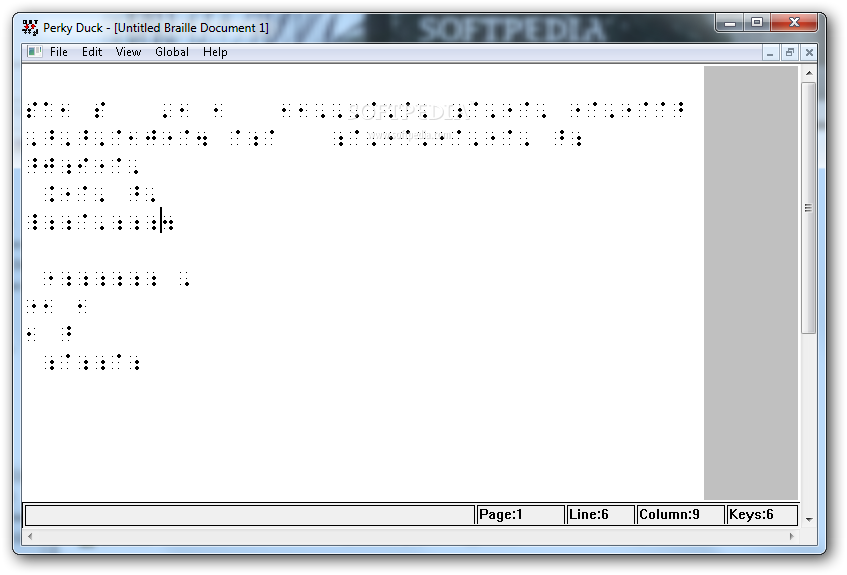
\includegraphics[scale=0.5]{ch02/assets/perky-duck-gui.png}
    \decoRule
    \caption[Interface do Perky Duck]{Interface do Perky Duck}
    \label{fig:ch02-perky-duck-gui}
\end{figure}

Disponível para Windows e MAC OS, a aplicação replica as características táteis da máquina braille, permitindo que os usuários experimentem virtualmente o processo de criação de documentos em braille. Para garantir uma experiência inclusiva, o Perky Duck fornece feedback auditivo e visual durante o uso. Isso inclui sons indicativos de progresso, juntamente com visualização na tela para acompanhar a tradução de texto para braille. 

Os usuários podem selecionar diferentes tipos de braille, ajustar o espaçamento entre células, definir configurações de formatação e entre outros, para atender às suas preferências individuais e requisitos específicos.

\subsection{Accessibyte: Braillio}

Braillio é uma aplicação web paga, projetada para auxiliar no aprendizado de Braille e da Máquina Braille. A aplicação pode ser acessada através de dispositivos móveis.

Uma característica central da aplicação é a simulação tátil e sonora da máquina Braille. Ao interagir com a aplicação, os usuários experimentam a sensação realista de pressionar as teclas da máquina Braille, acompanhada por sons que imitam o mecanismo de impressão. Isso proporciona uma experiência imersiva que ajuda os usuários a entender e memorizar a disposição dos pontos Braille. Os usuários recebem pistas auditivas, feedback tátil através de vibrações na tela (se estiverem usando um dispositivo touchscreen) e prompts visuais para reforçar sua compreensão dos caracteres e padrões Braille. Essa abordagem multissensorial atende a diferentes estilos de aprendizado e promove a retenção.

\begin{figure}[h]
    \centering
    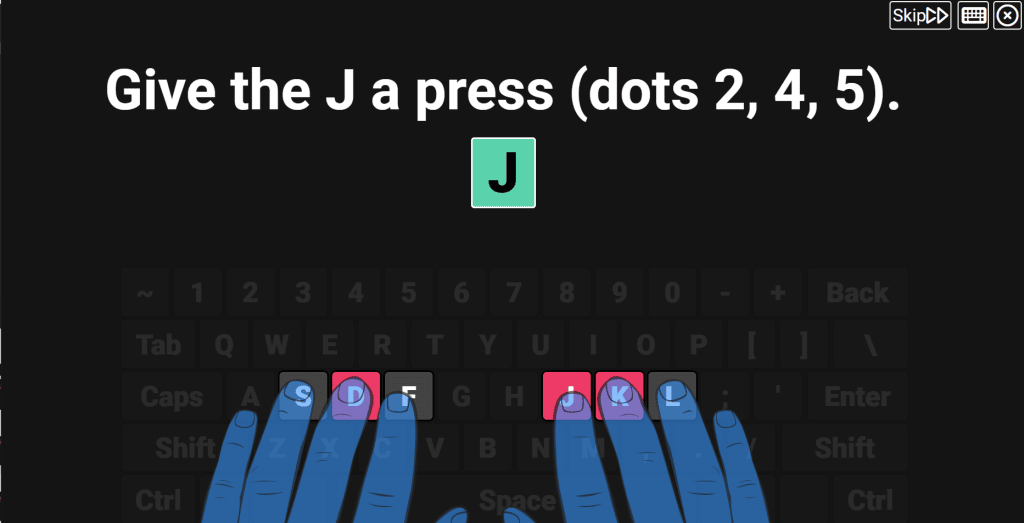
\includegraphics[scale=0.3]{ch02/assets/braillio-gui.png}
    \decoRule
    \caption[Interface do Braillio]{Interface do Braillio}
    \label{fig:ch02-braillio-gui}
\end{figure}

O Braillio oferece uma série de lições interativas que guiam os usuários pelos fundamentos do Braille. Essas lições são cuidadosamente estruturadas para introduzir gradualmente o alfabeto Braille, contrações, pontuação e mais. Cada lição incorpora instruções de áudio, feedback tátil e exercícios interativos para reforçar a aprendizagem. Com uma interface intuitiva e fácil de usar, torna a prática do Braille acessível a iniciantes e usuários avançados. 

Os usuários podem praticar a digitação de caracteres individuais, palavras e frases completas, recebendo feedback instantâneo sobre sua precisão e velocidade. Isso facilita a prática regular e o aprimoramento das habilidades em Braille.


\section{Desafios e Oportunidades}

Garantir que a simulação da máquina de escrever em Braille seja fiel à experiência real é um grande desafio a se enfrentar. Isso inclui replicar com precisão as sensações táteis e sonoras associadas ao uso da máquina, garantindo uma experiência imersiva e autêntica para os usuários. Embora deva oferecer um feedback auditivo e visual durante o uso, garantir a acessibilidade para usuários com diferentes necessidades sensoriais pode ser difícil. Isso inclui fornecer opções para usuários surdos ou com deficiência auditiva, bem como aqueles com limitações visuais.

Os simuladores precisam atender às necessidades de uma ampla gama de usuários, desde iniciantes no Braille até usuários avançados. Isso requer a implementação de recursos que sejam intuitivos para iniciantes, mas também desafiadores e personalizáveis para usuários mais experientes. Além de oferecer lições e exercícios que guiem os usuários desde os fundamentos básicos até habilidades mais avançadas, garantindo uma curva de aprendizado suave e eficiente.

Com o advento da tecnologia web, os simuladores podem ser acessados em uma variedade de dispositivos, incluindo computadores, tablets e smartphones. Isso aumenta sua acessibilidade global, permitindo que mais pessoas em diferentes contextos e localizações geográficas acessem as ferramentas de aprendizado do Braille. Podendo servir como plataformas para colaboração e comunidade, permitindo que os usuários compartilhem recursos, dicas e experiências de aprendizado. Isso cria um ambiente de apoio e colaboração entre os aprendizes de Braille, promovendo uma abordagem de aprendizado social e engajada.

\section{Comparativo entre aplicações}

% Após análise das aplicações vemos que em sua maioria são aplicações gratuitas. Porém apenas duas são web, as outras aplicação são da plataforma Android, Windows ou MAC. O problema de 

\begin{table}[h]
    \caption{Comparativo de aplicações}
    \label{tab:ch02-comparative}
    \centering
    \begin{tabular}{llcc}
        \toprule
        \tabhead{Aplicação}&  \tabhead{Plataforma}&  \tabhead{É gratuita?}& \tabhead{Ensina Braille?}\\
        \midrule
        BrailleType&  Android&  Sim& Não\\
        \addlinespace
        SingleTapBraille&  Android&  Sim& Não\\
        \addlinespace
        Brailendo&  Windows&  Sim& Sim\\
        \addlinespace
        Braillearnig&  Windows&  Sim& Sim\\
        \addlinespace
        Braille Fácil&  Windows&  Sim& Não\\
        \addlinespace
        Perky Duck&  Windows e MAC&  Sim& Não\\
        \addlinespace
        Braillio&  Web&  Não& Sim\\
        \addlinespace
        SWBraille& Web& Sim&Sim\\
        \bottomrule\\
    \end{tabular}
\end{table}

